% Graphic for TeX using PGF
% Title: /home/racine/Documents/Diagramme BDD/diagrammeBBDfinal.dia
% Creator: Dia v0.97.2
% CreationDate: Mon May 20 11:44:39 2013
% For: racine
% \usepackage{tikz}
% The following commands are not supported in PSTricks at present
% We define them conditionally, so when they are implemented,
% this pgf file will use them.
\ifx\du\undefined
  \newlength{\du}
\fi
\setlength{\du}{15\unitlength}
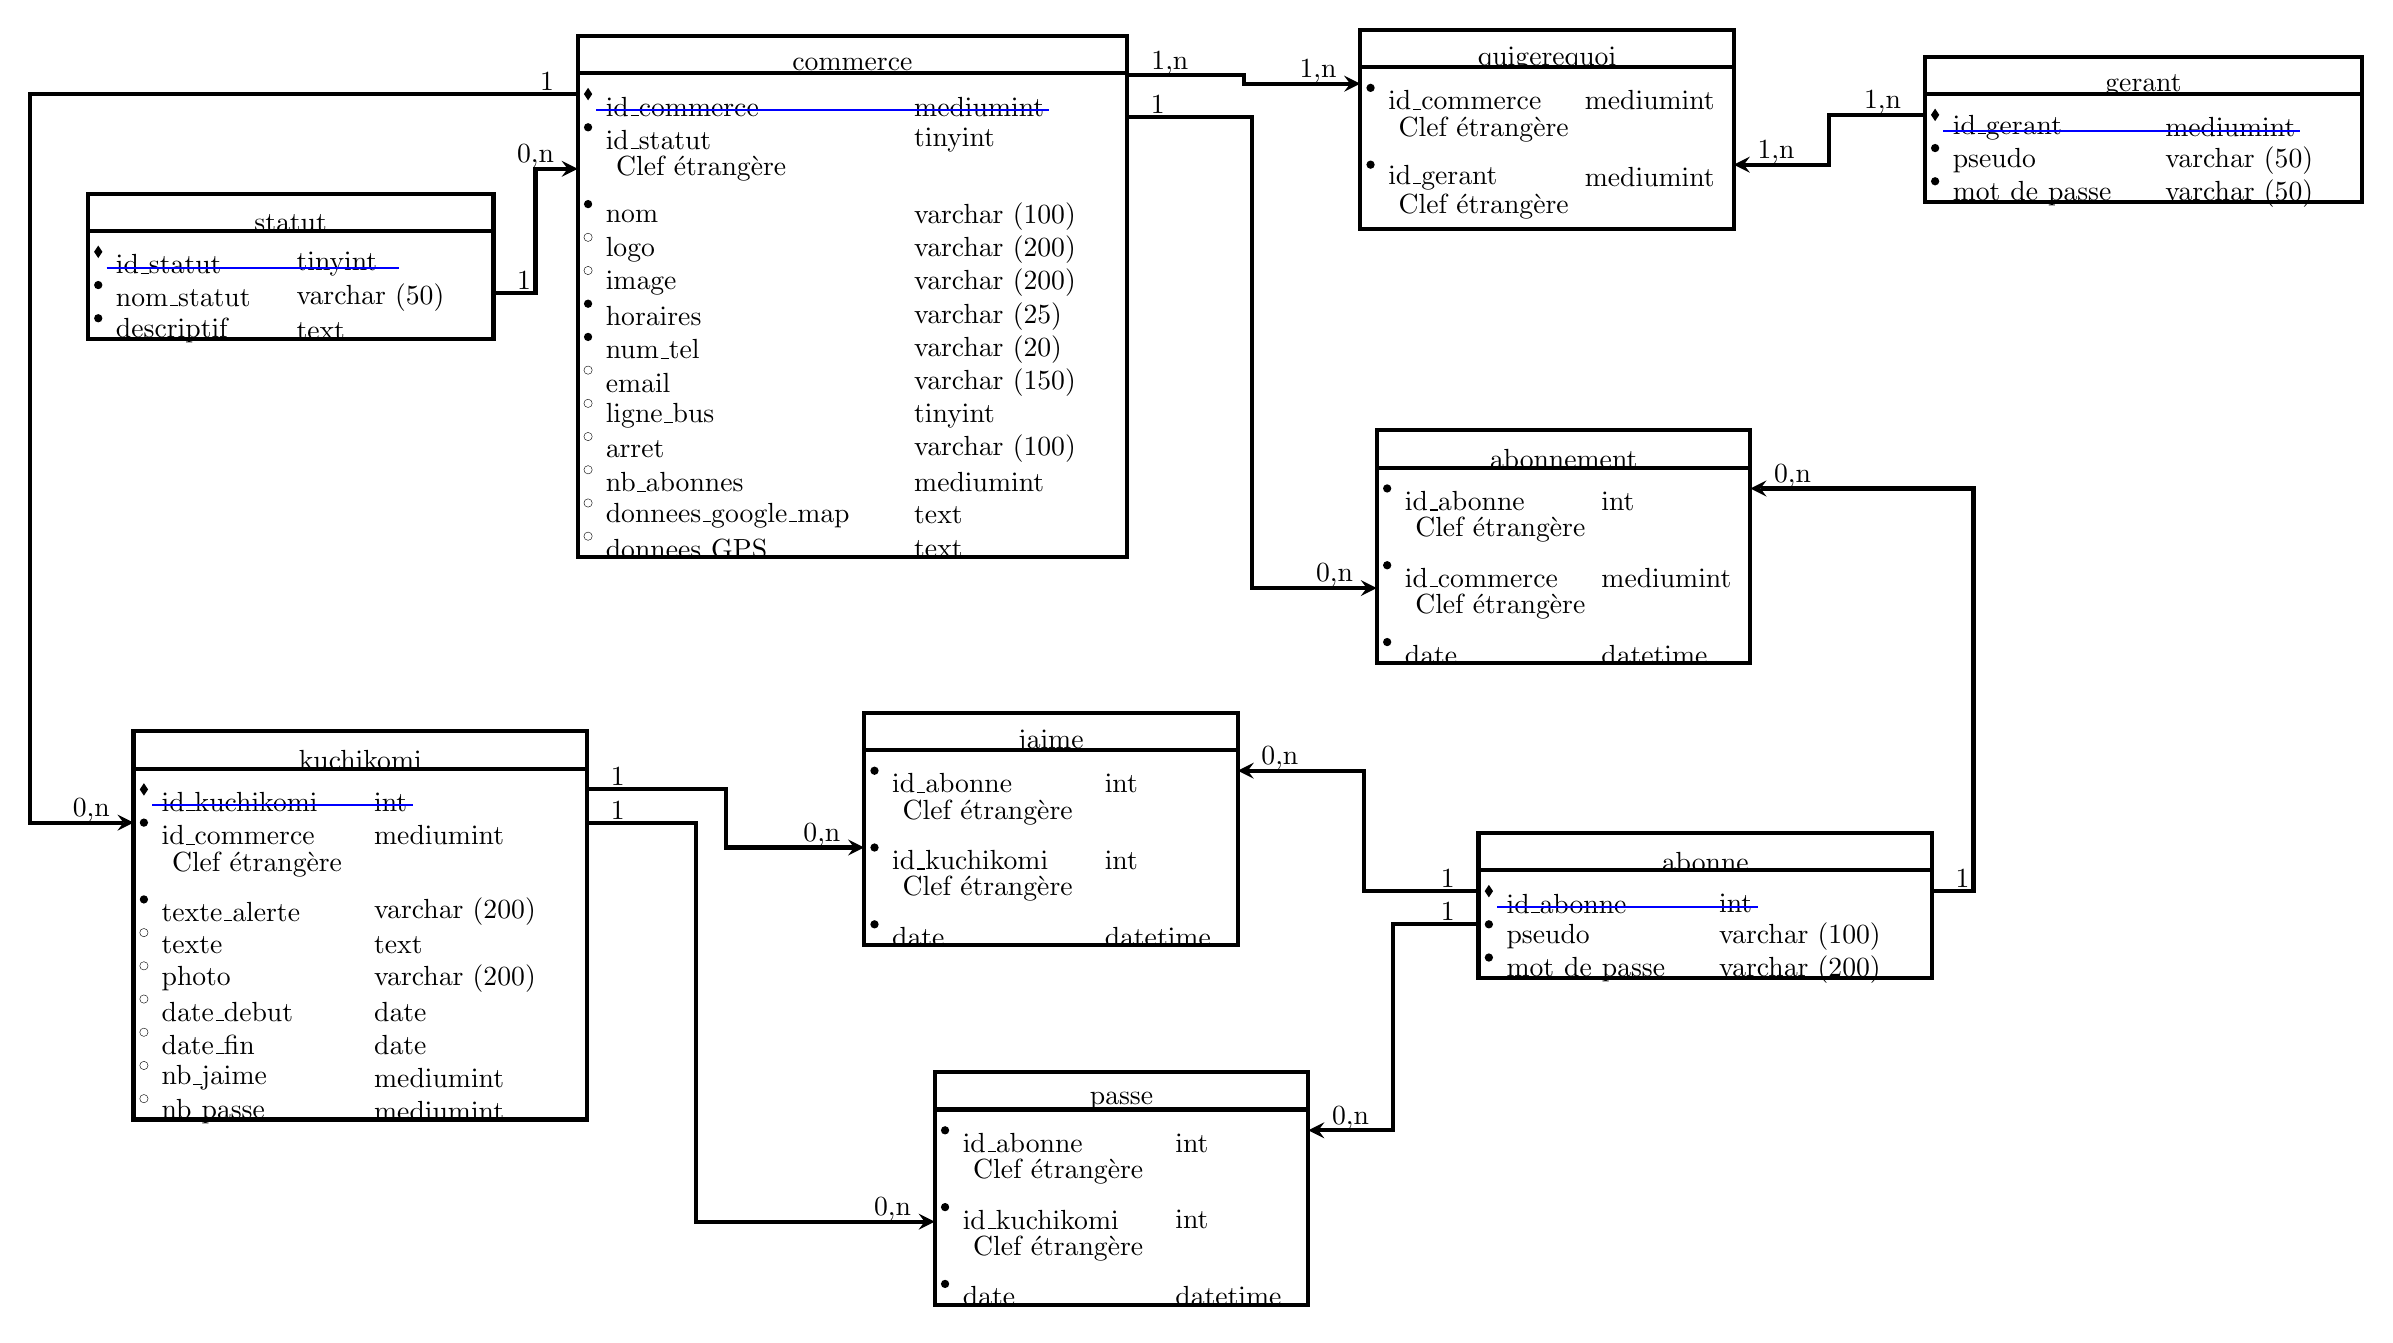
\begin{tikzpicture}
\pgftransformxscale{1.000000}
\pgftransformyscale{-1.000000}
\definecolor{dialinecolor}{rgb}{0.000000, 0.000000, 0.000000}
\pgfsetstrokecolor{dialinecolor}
\definecolor{dialinecolor}{rgb}{1.000000, 1.000000, 1.000000}
\pgfsetfillcolor{dialinecolor}
\pgfsetlinewidth{0.100000\du}
\pgfsetdash{}{0pt}
\definecolor{dialinecolor}{rgb}{1.000000, 1.000000, 1.000000}
\pgfsetfillcolor{dialinecolor}
\fill (15.450000\du,1.450000\du)--(15.450000\du,2.350000\du)--(28.685000\du,2.350000\du)--(28.685000\du,1.450000\du)--cycle;
\definecolor{dialinecolor}{rgb}{0.000000, 0.000000, 0.000000}
\pgfsetstrokecolor{dialinecolor}
\draw (15.450000\du,1.450000\du)--(15.450000\du,2.350000\du)--(28.685000\du,2.350000\du)--(28.685000\du,1.450000\du)--cycle;
% setfont left to latex
\definecolor{dialinecolor}{rgb}{0.000000, 0.000000, 1.000000}
\pgfsetstrokecolor{dialinecolor}
\node at (22.067500\du,2.150000\du){commerce};
\definecolor{dialinecolor}{rgb}{1.000000, 1.000000, 1.000000}
\pgfsetfillcolor{dialinecolor}
\fill (15.450000\du,2.350000\du)--(15.450000\du,14.000000\du)--(28.685000\du,14.000000\du)--(28.685000\du,2.350000\du)--cycle;
\definecolor{dialinecolor}{rgb}{0.000000, 0.000000, 0.000000}
\pgfsetstrokecolor{dialinecolor}
\draw (15.450000\du,2.350000\du)--(15.450000\du,14.000000\du)--(28.685000\du,14.000000\du)--(28.685000\du,2.350000\du)--cycle;
% setfont left to latex
\pgfsetlinewidth{0.010000\du}
\pgfsetmiterjoin
\definecolor{dialinecolor}{rgb}{0.000000, 0.000000, 0.000000}
\pgfsetfillcolor{dialinecolor}
\fill (15.600000\du,2.850000\du)--(15.700000\du,3.000000\du)--(15.800000\du,2.850000\du)--(15.700000\du,2.700000\du)--cycle;
\definecolor{dialinecolor}{rgb}{0.000000, 0.000000, 1.000000}
\pgfsetstrokecolor{dialinecolor}
\node[anchor=west] at (15.900000\du,3.150000\du){id\_commerce};
\definecolor{dialinecolor}{rgb}{0.000000, 0.000000, 1.000000}
\pgfsetstrokecolor{dialinecolor}
\node[anchor=west] at (23.330000\du,3.150000\du){mediumint};
\pgfsetlinewidth{0.050000\du}
\definecolor{dialinecolor}{rgb}{0.000000, 0.000000, 1.000000}
\pgfsetstrokecolor{dialinecolor}
\draw (15.900000\du,3.230000\du)--(26.795000\du,3.230000\du);
% setfont left to latex
\pgfsetlinewidth{0.010000\du}
\definecolor{dialinecolor}{rgb}{0.000000, 0.000000, 0.000000}
\pgfsetfillcolor{dialinecolor}
\pgfpathellipse{\pgfpoint{15.700000\du}{3.650000\du}}{\pgfpoint{0.100000\du}{0\du}}{\pgfpoint{0\du}{0.100000\du}}
\pgfusepath{fill}
\definecolor{dialinecolor}{rgb}{0.000000, 0.000000, 1.000000}
\pgfsetstrokecolor{dialinecolor}
\node[anchor=west] at (15.900000\du,3.950000\du){id\_statut};
\definecolor{dialinecolor}{rgb}{0.000000, 0.000000, 1.000000}
\pgfsetstrokecolor{dialinecolor}
\node[anchor=west] at (23.330000\du,3.950000\du){tinyint};
% setfont left to latex
\definecolor{dialinecolor}{rgb}{0.000000, 0.000000, 1.000000}
\pgfsetstrokecolor{dialinecolor}
\node[anchor=west] at (16.150000\du,4.650000\du){Clef étrangère};
% setfont left to latex
\pgfsetlinewidth{0.010000\du}
\definecolor{dialinecolor}{rgb}{0.000000, 0.000000, 0.000000}
\pgfsetfillcolor{dialinecolor}
\pgfpathellipse{\pgfpoint{15.700000\du}{5.500000\du}}{\pgfpoint{0.100000\du}{0\du}}{\pgfpoint{0\du}{0.100000\du}}
\pgfusepath{fill}
\definecolor{dialinecolor}{rgb}{0.000000, 0.000000, 1.000000}
\pgfsetstrokecolor{dialinecolor}
\node[anchor=west] at (15.900000\du,5.800000\du){nom};
\definecolor{dialinecolor}{rgb}{0.000000, 0.000000, 1.000000}
\pgfsetstrokecolor{dialinecolor}
\node[anchor=west] at (23.330000\du,5.800000\du){varchar (100)};
% setfont left to latex
\pgfsetlinewidth{0.010000\du}
\definecolor{dialinecolor}{rgb}{0.000000, 0.000000, 0.000000}
\pgfsetstrokecolor{dialinecolor}
\pgfpathellipse{\pgfpoint{15.700000\du}{6.300000\du}}{\pgfpoint{0.100000\du}{0\du}}{\pgfpoint{0\du}{0.100000\du}}
\pgfusepath{stroke}
\definecolor{dialinecolor}{rgb}{0.000000, 0.000000, 1.000000}
\pgfsetstrokecolor{dialinecolor}
\node[anchor=west] at (15.900000\du,6.600000\du){logo};
\definecolor{dialinecolor}{rgb}{0.000000, 0.000000, 1.000000}
\pgfsetstrokecolor{dialinecolor}
\node[anchor=west] at (23.330000\du,6.600000\du){varchar (200)};
% setfont left to latex
\pgfsetlinewidth{0.010000\du}
\definecolor{dialinecolor}{rgb}{0.000000, 0.000000, 0.000000}
\pgfsetstrokecolor{dialinecolor}
\pgfpathellipse{\pgfpoint{15.700000\du}{7.100000\du}}{\pgfpoint{0.100000\du}{0\du}}{\pgfpoint{0\du}{0.100000\du}}
\pgfusepath{stroke}
\definecolor{dialinecolor}{rgb}{0.000000, 0.000000, 1.000000}
\pgfsetstrokecolor{dialinecolor}
\node[anchor=west] at (15.900000\du,7.400000\du){image};
\definecolor{dialinecolor}{rgb}{0.000000, 0.000000, 1.000000}
\pgfsetstrokecolor{dialinecolor}
\node[anchor=west] at (23.330000\du,7.400000\du){varchar (200)};
% setfont left to latex
\pgfsetlinewidth{0.010000\du}
\definecolor{dialinecolor}{rgb}{0.000000, 0.000000, 0.000000}
\pgfsetfillcolor{dialinecolor}
\pgfpathellipse{\pgfpoint{15.700000\du}{7.900000\du}}{\pgfpoint{0.100000\du}{0\du}}{\pgfpoint{0\du}{0.100000\du}}
\pgfusepath{fill}
\definecolor{dialinecolor}{rgb}{0.000000, 0.000000, 1.000000}
\pgfsetstrokecolor{dialinecolor}
\node[anchor=west] at (15.900000\du,8.200000\du){horaires};
\definecolor{dialinecolor}{rgb}{0.000000, 0.000000, 1.000000}
\pgfsetstrokecolor{dialinecolor}
\node[anchor=west] at (23.330000\du,8.200000\du){varchar (25)};
% setfont left to latex
\pgfsetlinewidth{0.010000\du}
\definecolor{dialinecolor}{rgb}{0.000000, 0.000000, 0.000000}
\pgfsetfillcolor{dialinecolor}
\pgfpathellipse{\pgfpoint{15.700000\du}{8.700000\du}}{\pgfpoint{0.100000\du}{0\du}}{\pgfpoint{0\du}{0.100000\du}}
\pgfusepath{fill}
\definecolor{dialinecolor}{rgb}{0.000000, 0.000000, 1.000000}
\pgfsetstrokecolor{dialinecolor}
\node[anchor=west] at (15.900000\du,9.000000\du){num\_tel};
\definecolor{dialinecolor}{rgb}{0.000000, 0.000000, 1.000000}
\pgfsetstrokecolor{dialinecolor}
\node[anchor=west] at (23.330000\du,9.000000\du){varchar (20)};
% setfont left to latex
\pgfsetlinewidth{0.010000\du}
\definecolor{dialinecolor}{rgb}{0.000000, 0.000000, 0.000000}
\pgfsetstrokecolor{dialinecolor}
\pgfpathellipse{\pgfpoint{15.700000\du}{9.500000\du}}{\pgfpoint{0.100000\du}{0\du}}{\pgfpoint{0\du}{0.100000\du}}
\pgfusepath{stroke}
\definecolor{dialinecolor}{rgb}{0.000000, 0.000000, 1.000000}
\pgfsetstrokecolor{dialinecolor}
\node[anchor=west] at (15.900000\du,9.800000\du){email};
\definecolor{dialinecolor}{rgb}{0.000000, 0.000000, 1.000000}
\pgfsetstrokecolor{dialinecolor}
\node[anchor=west] at (23.330000\du,9.800000\du){varchar (150)};
% setfont left to latex
\pgfsetlinewidth{0.010000\du}
\definecolor{dialinecolor}{rgb}{0.000000, 0.000000, 0.000000}
\pgfsetstrokecolor{dialinecolor}
\pgfpathellipse{\pgfpoint{15.700000\du}{10.300000\du}}{\pgfpoint{0.100000\du}{0\du}}{\pgfpoint{0\du}{0.100000\du}}
\pgfusepath{stroke}
\definecolor{dialinecolor}{rgb}{0.000000, 0.000000, 1.000000}
\pgfsetstrokecolor{dialinecolor}
\node[anchor=west] at (15.900000\du,10.600000\du){ligne\_bus};
\definecolor{dialinecolor}{rgb}{0.000000, 0.000000, 1.000000}
\pgfsetstrokecolor{dialinecolor}
\node[anchor=west] at (23.330000\du,10.600000\du){tinyint};
% setfont left to latex
\pgfsetlinewidth{0.010000\du}
\definecolor{dialinecolor}{rgb}{0.000000, 0.000000, 0.000000}
\pgfsetstrokecolor{dialinecolor}
\pgfpathellipse{\pgfpoint{15.700000\du}{11.100000\du}}{\pgfpoint{0.100000\du}{0\du}}{\pgfpoint{0\du}{0.100000\du}}
\pgfusepath{stroke}
\definecolor{dialinecolor}{rgb}{0.000000, 0.000000, 1.000000}
\pgfsetstrokecolor{dialinecolor}
\node[anchor=west] at (15.900000\du,11.400000\du){arret};
\definecolor{dialinecolor}{rgb}{0.000000, 0.000000, 1.000000}
\pgfsetstrokecolor{dialinecolor}
\node[anchor=west] at (23.330000\du,11.400000\du){varchar (100)};
% setfont left to latex
\pgfsetlinewidth{0.010000\du}
\definecolor{dialinecolor}{rgb}{0.000000, 0.000000, 0.000000}
\pgfsetstrokecolor{dialinecolor}
\pgfpathellipse{\pgfpoint{15.700000\du}{11.900000\du}}{\pgfpoint{0.100000\du}{0\du}}{\pgfpoint{0\du}{0.100000\du}}
\pgfusepath{stroke}
\definecolor{dialinecolor}{rgb}{0.000000, 0.000000, 1.000000}
\pgfsetstrokecolor{dialinecolor}
\node[anchor=west] at (15.900000\du,12.200000\du){nb\_abonnes};
\definecolor{dialinecolor}{rgb}{0.000000, 0.000000, 1.000000}
\pgfsetstrokecolor{dialinecolor}
\node[anchor=west] at (23.330000\du,12.200000\du){mediumint};
% setfont left to latex
\pgfsetlinewidth{0.010000\du}
\definecolor{dialinecolor}{rgb}{0.000000, 0.000000, 0.000000}
\pgfsetstrokecolor{dialinecolor}
\pgfpathellipse{\pgfpoint{15.700000\du}{12.700000\du}}{\pgfpoint{0.100000\du}{0\du}}{\pgfpoint{0\du}{0.100000\du}}
\pgfusepath{stroke}
\definecolor{dialinecolor}{rgb}{0.000000, 0.000000, 1.000000}
\pgfsetstrokecolor{dialinecolor}
\node[anchor=west] at (15.900000\du,13.000000\du){donnees\_google\_map};
\definecolor{dialinecolor}{rgb}{0.000000, 0.000000, 1.000000}
\pgfsetstrokecolor{dialinecolor}
\node[anchor=west] at (23.330000\du,13.000000\du){text};
% setfont left to latex
\pgfsetlinewidth{0.010000\du}
\definecolor{dialinecolor}{rgb}{0.000000, 0.000000, 0.000000}
\pgfsetstrokecolor{dialinecolor}
\pgfpathellipse{\pgfpoint{15.700000\du}{13.500000\du}}{\pgfpoint{0.100000\du}{0\du}}{\pgfpoint{0\du}{0.100000\du}}
\pgfusepath{stroke}
\definecolor{dialinecolor}{rgb}{0.000000, 0.000000, 1.000000}
\pgfsetstrokecolor{dialinecolor}
\node[anchor=west] at (15.900000\du,13.800000\du){donnees\_GPS};
\definecolor{dialinecolor}{rgb}{0.000000, 0.000000, 1.000000}
\pgfsetstrokecolor{dialinecolor}
\node[anchor=west] at (23.330000\du,13.800000\du){text};
\pgfsetlinewidth{0.100000\du}
\pgfsetdash{}{0pt}
\definecolor{dialinecolor}{rgb}{1.000000, 1.000000, 1.000000}
\pgfsetfillcolor{dialinecolor}
\fill (3.650000\du,5.250000\du)--(3.650000\du,6.150000\du)--(13.420000\du,6.150000\du)--(13.420000\du,5.250000\du)--cycle;
\definecolor{dialinecolor}{rgb}{0.000000, 0.000000, 0.000000}
\pgfsetstrokecolor{dialinecolor}
\draw (3.650000\du,5.250000\du)--(3.650000\du,6.150000\du)--(13.420000\du,6.150000\du)--(13.420000\du,5.250000\du)--cycle;
% setfont left to latex
\definecolor{dialinecolor}{rgb}{0.000000, 0.000000, 1.000000}
\pgfsetstrokecolor{dialinecolor}
\node at (8.535000\du,5.950000\du){statut};
\definecolor{dialinecolor}{rgb}{1.000000, 1.000000, 1.000000}
\pgfsetfillcolor{dialinecolor}
\fill (3.650000\du,6.150000\du)--(3.650000\du,8.750000\du)--(13.420000\du,8.750000\du)--(13.420000\du,6.150000\du)--cycle;
\definecolor{dialinecolor}{rgb}{0.000000, 0.000000, 0.000000}
\pgfsetstrokecolor{dialinecolor}
\draw (3.650000\du,6.150000\du)--(3.650000\du,8.750000\du)--(13.420000\du,8.750000\du)--(13.420000\du,6.150000\du)--cycle;
% setfont left to latex
\pgfsetlinewidth{0.010000\du}
\pgfsetmiterjoin
\definecolor{dialinecolor}{rgb}{0.000000, 0.000000, 0.000000}
\pgfsetfillcolor{dialinecolor}
\fill (3.800000\du,6.650000\du)--(3.900000\du,6.800000\du)--(4.000000\du,6.650000\du)--(3.900000\du,6.500000\du)--cycle;
\definecolor{dialinecolor}{rgb}{0.000000, 0.000000, 1.000000}
\pgfsetstrokecolor{dialinecolor}
\node[anchor=west] at (4.100000\du,6.950000\du){id\_statut};
\definecolor{dialinecolor}{rgb}{0.000000, 0.000000, 1.000000}
\pgfsetstrokecolor{dialinecolor}
\node[anchor=west] at (8.450000\du,6.950000\du){tinyint};
\pgfsetlinewidth{0.050000\du}
\definecolor{dialinecolor}{rgb}{0.000000, 0.000000, 1.000000}
\pgfsetstrokecolor{dialinecolor}
\draw (4.100000\du,7.030000\du)--(11.145000\du,7.030000\du);
% setfont left to latex
\pgfsetlinewidth{0.010000\du}
\definecolor{dialinecolor}{rgb}{0.000000, 0.000000, 0.000000}
\pgfsetfillcolor{dialinecolor}
\pgfpathellipse{\pgfpoint{3.900000\du}{7.450000\du}}{\pgfpoint{0.100000\du}{0\du}}{\pgfpoint{0\du}{0.100000\du}}
\pgfusepath{fill}
\definecolor{dialinecolor}{rgb}{0.000000, 0.000000, 1.000000}
\pgfsetstrokecolor{dialinecolor}
\node[anchor=west] at (4.100000\du,7.750000\du){nom\_statut};
\definecolor{dialinecolor}{rgb}{0.000000, 0.000000, 1.000000}
\pgfsetstrokecolor{dialinecolor}
\node[anchor=west] at (8.450000\du,7.750000\du){varchar (50)};
% setfont left to latex
\pgfsetlinewidth{0.010000\du}
\definecolor{dialinecolor}{rgb}{0.000000, 0.000000, 0.000000}
\pgfsetfillcolor{dialinecolor}
\pgfpathellipse{\pgfpoint{3.900000\du}{8.250000\du}}{\pgfpoint{0.100000\du}{0\du}}{\pgfpoint{0\du}{0.100000\du}}
\pgfusepath{fill}
\definecolor{dialinecolor}{rgb}{0.000000, 0.000000, 1.000000}
\pgfsetstrokecolor{dialinecolor}
\node[anchor=west] at (4.100000\du,8.550000\du){descriptif};
\definecolor{dialinecolor}{rgb}{0.000000, 0.000000, 1.000000}
\pgfsetstrokecolor{dialinecolor}
\node[anchor=west] at (8.450000\du,8.550000\du){text};
\pgfsetlinewidth{0.100000\du}
\pgfsetdash{}{0pt}
\definecolor{dialinecolor}{rgb}{1.000000, 1.000000, 1.000000}
\pgfsetfillcolor{dialinecolor}
\fill (34.300000\du,1.300000\du)--(34.300000\du,2.200000\du)--(43.300000\du,2.200000\du)--(43.300000\du,1.300000\du)--cycle;
\definecolor{dialinecolor}{rgb}{0.000000, 0.000000, 0.000000}
\pgfsetstrokecolor{dialinecolor}
\draw (34.300000\du,1.300000\du)--(34.300000\du,2.200000\du)--(43.300000\du,2.200000\du)--(43.300000\du,1.300000\du)--cycle;
% setfont left to latex
\definecolor{dialinecolor}{rgb}{0.000000, 0.000000, 1.000000}
\pgfsetstrokecolor{dialinecolor}
\node at (38.800000\du,2.000000\du){quigerequoi};
\definecolor{dialinecolor}{rgb}{1.000000, 1.000000, 1.000000}
\pgfsetfillcolor{dialinecolor}
\fill (34.300000\du,2.200000\du)--(34.300000\du,6.100000\du)--(43.300000\du,6.100000\du)--(43.300000\du,2.200000\du)--cycle;
\definecolor{dialinecolor}{rgb}{0.000000, 0.000000, 0.000000}
\pgfsetstrokecolor{dialinecolor}
\draw (34.300000\du,2.200000\du)--(34.300000\du,6.100000\du)--(43.300000\du,6.100000\du)--(43.300000\du,2.200000\du)--cycle;
% setfont left to latex
\pgfsetlinewidth{0.010000\du}
\definecolor{dialinecolor}{rgb}{0.000000, 0.000000, 0.000000}
\pgfsetfillcolor{dialinecolor}
\pgfpathellipse{\pgfpoint{34.550000\du}{2.700000\du}}{\pgfpoint{0.100000\du}{0\du}}{\pgfpoint{0\du}{0.100000\du}}
\pgfusepath{fill}
\definecolor{dialinecolor}{rgb}{0.000000, 0.000000, 1.000000}
\pgfsetstrokecolor{dialinecolor}
\node[anchor=west] at (34.750000\du,3.000000\du){id\_commerce};
\definecolor{dialinecolor}{rgb}{0.000000, 0.000000, 1.000000}
\pgfsetstrokecolor{dialinecolor}
\node[anchor=west] at (39.485000\du,3.000000\du){mediumint};
% setfont left to latex
\definecolor{dialinecolor}{rgb}{0.000000, 0.000000, 1.000000}
\pgfsetstrokecolor{dialinecolor}
\node[anchor=west] at (35.000000\du,3.700000\du){Clef étrangère};
% setfont left to latex
\pgfsetlinewidth{0.010000\du}
\definecolor{dialinecolor}{rgb}{0.000000, 0.000000, 0.000000}
\pgfsetfillcolor{dialinecolor}
\pgfpathellipse{\pgfpoint{34.550000\du}{4.550000\du}}{\pgfpoint{0.100000\du}{0\du}}{\pgfpoint{0\du}{0.100000\du}}
\pgfusepath{fill}
\definecolor{dialinecolor}{rgb}{0.000000, 0.000000, 1.000000}
\pgfsetstrokecolor{dialinecolor}
\node[anchor=west] at (34.750000\du,4.850000\du){id\_gerant};
\definecolor{dialinecolor}{rgb}{0.000000, 0.000000, 1.000000}
\pgfsetstrokecolor{dialinecolor}
\node[anchor=west] at (39.485000\du,4.850000\du){mediumint};
% setfont left to latex
\definecolor{dialinecolor}{rgb}{0.000000, 0.000000, 1.000000}
\pgfsetstrokecolor{dialinecolor}
\node[anchor=west] at (35.000000\du,5.550000\du){Clef étrangère};
\pgfsetlinewidth{0.100000\du}
\pgfsetdash{}{0pt}
\pgfsetdash{}{0pt}
\pgfsetmiterjoin
\pgfsetbuttcap
{
\definecolor{dialinecolor}{rgb}{0.000000, 0.000000, 0.000000}
\pgfsetfillcolor{dialinecolor}
% was here!!!
\pgfsetarrowsend{stealth}
{\pgfsetcornersarced{\pgfpoint{0.000000\du}{0.000000\du}}\definecolor{dialinecolor}{rgb}{0.000000, 0.000000, 0.000000}
\pgfsetstrokecolor{dialinecolor}
\draw (28.700000\du,2.400000\du)--(31.500000\du,2.400000\du)--(31.500000\du,2.600000\du)--(34.300000\du,2.600000\du);
}}
% setfont left to latex
\definecolor{dialinecolor}{rgb}{1.000000, 0.000000, 0.000000}
\pgfsetstrokecolor{dialinecolor}
\node[anchor=west] at (29.000000\du,2.100000\du){1,n};
\definecolor{dialinecolor}{rgb}{1.000000, 0.000000, 0.000000}
\pgfsetstrokecolor{dialinecolor}
\node[anchor=east] at (34.000000\du,2.300000\du){1,n};
\pgfsetlinewidth{0.100000\du}
\pgfsetdash{}{0pt}
\definecolor{dialinecolor}{rgb}{1.000000, 1.000000, 1.000000}
\pgfsetfillcolor{dialinecolor}
\fill (47.900000\du,1.950000\du)--(47.900000\du,2.850000\du)--(58.440000\du,2.850000\du)--(58.440000\du,1.950000\du)--cycle;
\definecolor{dialinecolor}{rgb}{0.000000, 0.000000, 0.000000}
\pgfsetstrokecolor{dialinecolor}
\draw (47.900000\du,1.950000\du)--(47.900000\du,2.850000\du)--(58.440000\du,2.850000\du)--(58.440000\du,1.950000\du)--cycle;
% setfont left to latex
\definecolor{dialinecolor}{rgb}{0.000000, 0.000000, 1.000000}
\pgfsetstrokecolor{dialinecolor}
\node at (53.170000\du,2.650000\du){gerant};
\definecolor{dialinecolor}{rgb}{1.000000, 1.000000, 1.000000}
\pgfsetfillcolor{dialinecolor}
\fill (47.900000\du,2.850000\du)--(47.900000\du,5.450000\du)--(58.440000\du,5.450000\du)--(58.440000\du,2.850000\du)--cycle;
\definecolor{dialinecolor}{rgb}{0.000000, 0.000000, 0.000000}
\pgfsetstrokecolor{dialinecolor}
\draw (47.900000\du,2.850000\du)--(47.900000\du,5.450000\du)--(58.440000\du,5.450000\du)--(58.440000\du,2.850000\du)--cycle;
% setfont left to latex
\pgfsetlinewidth{0.010000\du}
\pgfsetmiterjoin
\definecolor{dialinecolor}{rgb}{0.000000, 0.000000, 0.000000}
\pgfsetfillcolor{dialinecolor}
\fill (48.050000\du,3.350000\du)--(48.150000\du,3.500000\du)--(48.250000\du,3.350000\du)--(48.150000\du,3.200000\du)--cycle;
\definecolor{dialinecolor}{rgb}{0.000000, 0.000000, 1.000000}
\pgfsetstrokecolor{dialinecolor}
\node[anchor=west] at (48.350000\du,3.650000\du){id\_gerant};
\definecolor{dialinecolor}{rgb}{0.000000, 0.000000, 1.000000}
\pgfsetstrokecolor{dialinecolor}
\node[anchor=west] at (53.470000\du,3.650000\du){mediumint};
\pgfsetlinewidth{0.050000\du}
\definecolor{dialinecolor}{rgb}{0.000000, 0.000000, 1.000000}
\pgfsetstrokecolor{dialinecolor}
\draw (48.350000\du,3.730000\du)--(56.935000\du,3.730000\du);
% setfont left to latex
\pgfsetlinewidth{0.010000\du}
\definecolor{dialinecolor}{rgb}{0.000000, 0.000000, 0.000000}
\pgfsetfillcolor{dialinecolor}
\pgfpathellipse{\pgfpoint{48.150000\du}{4.150000\du}}{\pgfpoint{0.100000\du}{0\du}}{\pgfpoint{0\du}{0.100000\du}}
\pgfusepath{fill}
\definecolor{dialinecolor}{rgb}{0.000000, 0.000000, 1.000000}
\pgfsetstrokecolor{dialinecolor}
\node[anchor=west] at (48.350000\du,4.450000\du){pseudo};
\definecolor{dialinecolor}{rgb}{0.000000, 0.000000, 1.000000}
\pgfsetstrokecolor{dialinecolor}
\node[anchor=west] at (53.470000\du,4.450000\du){varchar (50)};
% setfont left to latex
\pgfsetlinewidth{0.010000\du}
\definecolor{dialinecolor}{rgb}{0.000000, 0.000000, 0.000000}
\pgfsetfillcolor{dialinecolor}
\pgfpathellipse{\pgfpoint{48.150000\du}{4.950000\du}}{\pgfpoint{0.100000\du}{0\du}}{\pgfpoint{0\du}{0.100000\du}}
\pgfusepath{fill}
\definecolor{dialinecolor}{rgb}{0.000000, 0.000000, 1.000000}
\pgfsetstrokecolor{dialinecolor}
\node[anchor=west] at (48.350000\du,5.250000\du){mot\_de\_passe};
\definecolor{dialinecolor}{rgb}{0.000000, 0.000000, 1.000000}
\pgfsetstrokecolor{dialinecolor}
\node[anchor=west] at (53.470000\du,5.250000\du){varchar (50)};
\pgfsetlinewidth{0.100000\du}
\pgfsetdash{}{0pt}
\pgfsetdash{}{0pt}
\pgfsetmiterjoin
\pgfsetbuttcap
{
\definecolor{dialinecolor}{rgb}{0.000000, 0.000000, 0.000000}
\pgfsetfillcolor{dialinecolor}
% was here!!!
\pgfsetarrowsend{stealth}
{\pgfsetcornersarced{\pgfpoint{0.000000\du}{0.000000\du}}\definecolor{dialinecolor}{rgb}{0.000000, 0.000000, 0.000000}
\pgfsetstrokecolor{dialinecolor}
\draw (47.900000\du,3.350000\du)--(45.600000\du,3.350000\du)--(45.600000\du,4.550000\du)--(43.300000\du,4.550000\du);
}}
% setfont left to latex
\definecolor{dialinecolor}{rgb}{1.000000, 0.000000, 0.000000}
\pgfsetstrokecolor{dialinecolor}
\node[anchor=east] at (47.600000\du,3.050000\du){1,n};
\definecolor{dialinecolor}{rgb}{1.000000, 0.000000, 0.000000}
\pgfsetstrokecolor{dialinecolor}
\node[anchor=west] at (43.600000\du,4.250000\du){1,n};
\pgfsetlinewidth{0.100000\du}
\pgfsetdash{}{0pt}
\definecolor{dialinecolor}{rgb}{1.000000, 1.000000, 1.000000}
\pgfsetfillcolor{dialinecolor}
\fill (4.750000\du,18.200000\du)--(4.750000\du,19.100000\du)--(15.675000\du,19.100000\du)--(15.675000\du,18.200000\du)--cycle;
\definecolor{dialinecolor}{rgb}{0.000000, 0.000000, 0.000000}
\pgfsetstrokecolor{dialinecolor}
\draw (4.750000\du,18.200000\du)--(4.750000\du,19.100000\du)--(15.675000\du,19.100000\du)--(15.675000\du,18.200000\du)--cycle;
% setfont left to latex
\definecolor{dialinecolor}{rgb}{0.000000, 0.000000, 1.000000}
\pgfsetstrokecolor{dialinecolor}
\node at (10.212500\du,18.900000\du){kuchikomi};
\definecolor{dialinecolor}{rgb}{1.000000, 1.000000, 1.000000}
\pgfsetfillcolor{dialinecolor}
\fill (4.750000\du,19.100000\du)--(4.750000\du,27.550000\du)--(15.675000\du,27.550000\du)--(15.675000\du,19.100000\du)--cycle;
\definecolor{dialinecolor}{rgb}{0.000000, 0.000000, 0.000000}
\pgfsetstrokecolor{dialinecolor}
\draw (4.750000\du,19.100000\du)--(4.750000\du,27.550000\du)--(15.675000\du,27.550000\du)--(15.675000\du,19.100000\du)--cycle;
% setfont left to latex
\pgfsetlinewidth{0.010000\du}
\pgfsetmiterjoin
\definecolor{dialinecolor}{rgb}{0.000000, 0.000000, 0.000000}
\pgfsetfillcolor{dialinecolor}
\fill (4.900000\du,19.600000\du)--(5.000000\du,19.750000\du)--(5.100000\du,19.600000\du)--(5.000000\du,19.450000\du)--cycle;
\definecolor{dialinecolor}{rgb}{0.000000, 0.000000, 1.000000}
\pgfsetstrokecolor{dialinecolor}
\node[anchor=west] at (5.200000\du,19.900000\du){id\_kuchikomi};
\definecolor{dialinecolor}{rgb}{0.000000, 0.000000, 1.000000}
\pgfsetstrokecolor{dialinecolor}
\node[anchor=west] at (10.320000\du,19.900000\du){int};
\pgfsetlinewidth{0.050000\du}
\definecolor{dialinecolor}{rgb}{0.000000, 0.000000, 1.000000}
\pgfsetstrokecolor{dialinecolor}
\draw (5.200000\du,19.980000\du)--(11.475000\du,19.980000\du);
% setfont left to latex
\pgfsetlinewidth{0.010000\du}
\definecolor{dialinecolor}{rgb}{0.000000, 0.000000, 0.000000}
\pgfsetfillcolor{dialinecolor}
\pgfpathellipse{\pgfpoint{5.000000\du}{20.400000\du}}{\pgfpoint{0.100000\du}{0\du}}{\pgfpoint{0\du}{0.100000\du}}
\pgfusepath{fill}
\definecolor{dialinecolor}{rgb}{0.000000, 0.000000, 1.000000}
\pgfsetstrokecolor{dialinecolor}
\node[anchor=west] at (5.200000\du,20.700000\du){id\_commerce};
\definecolor{dialinecolor}{rgb}{0.000000, 0.000000, 1.000000}
\pgfsetstrokecolor{dialinecolor}
\node[anchor=west] at (10.320000\du,20.700000\du){mediumint};
% setfont left to latex
\definecolor{dialinecolor}{rgb}{0.000000, 0.000000, 1.000000}
\pgfsetstrokecolor{dialinecolor}
\node[anchor=west] at (5.450000\du,21.400000\du){Clef étrangère};
% setfont left to latex
\pgfsetlinewidth{0.010000\du}
\definecolor{dialinecolor}{rgb}{0.000000, 0.000000, 0.000000}
\pgfsetfillcolor{dialinecolor}
\pgfpathellipse{\pgfpoint{5.000000\du}{22.250000\du}}{\pgfpoint{0.100000\du}{0\du}}{\pgfpoint{0\du}{0.100000\du}}
\pgfusepath{fill}
\definecolor{dialinecolor}{rgb}{0.000000, 0.000000, 1.000000}
\pgfsetstrokecolor{dialinecolor}
\node[anchor=west] at (5.200000\du,22.550000\du){texte\_alerte};
\definecolor{dialinecolor}{rgb}{0.000000, 0.000000, 1.000000}
\pgfsetstrokecolor{dialinecolor}
\node[anchor=west] at (10.320000\du,22.550000\du){varchar (200)};
% setfont left to latex
\pgfsetlinewidth{0.010000\du}
\definecolor{dialinecolor}{rgb}{0.000000, 0.000000, 0.000000}
\pgfsetstrokecolor{dialinecolor}
\pgfpathellipse{\pgfpoint{5.000000\du}{23.050000\du}}{\pgfpoint{0.100000\du}{0\du}}{\pgfpoint{0\du}{0.100000\du}}
\pgfusepath{stroke}
\definecolor{dialinecolor}{rgb}{0.000000, 0.000000, 1.000000}
\pgfsetstrokecolor{dialinecolor}
\node[anchor=west] at (5.200000\du,23.350000\du){texte};
\definecolor{dialinecolor}{rgb}{0.000000, 0.000000, 1.000000}
\pgfsetstrokecolor{dialinecolor}
\node[anchor=west] at (10.320000\du,23.350000\du){text};
% setfont left to latex
\pgfsetlinewidth{0.010000\du}
\definecolor{dialinecolor}{rgb}{0.000000, 0.000000, 0.000000}
\pgfsetstrokecolor{dialinecolor}
\pgfpathellipse{\pgfpoint{5.000000\du}{23.850000\du}}{\pgfpoint{0.100000\du}{0\du}}{\pgfpoint{0\du}{0.100000\du}}
\pgfusepath{stroke}
\definecolor{dialinecolor}{rgb}{0.000000, 0.000000, 1.000000}
\pgfsetstrokecolor{dialinecolor}
\node[anchor=west] at (5.200000\du,24.150000\du){photo};
\definecolor{dialinecolor}{rgb}{0.000000, 0.000000, 1.000000}
\pgfsetstrokecolor{dialinecolor}
\node[anchor=west] at (10.320000\du,24.150000\du){varchar (200)};
% setfont left to latex
\pgfsetlinewidth{0.010000\du}
\definecolor{dialinecolor}{rgb}{0.000000, 0.000000, 0.000000}
\pgfsetstrokecolor{dialinecolor}
\pgfpathellipse{\pgfpoint{5.000000\du}{24.650000\du}}{\pgfpoint{0.100000\du}{0\du}}{\pgfpoint{0\du}{0.100000\du}}
\pgfusepath{stroke}
\definecolor{dialinecolor}{rgb}{0.000000, 0.000000, 1.000000}
\pgfsetstrokecolor{dialinecolor}
\node[anchor=west] at (5.200000\du,24.950000\du){date\_debut};
\definecolor{dialinecolor}{rgb}{0.000000, 0.000000, 1.000000}
\pgfsetstrokecolor{dialinecolor}
\node[anchor=west] at (10.320000\du,24.950000\du){date};
% setfont left to latex
\pgfsetlinewidth{0.010000\du}
\definecolor{dialinecolor}{rgb}{0.000000, 0.000000, 0.000000}
\pgfsetstrokecolor{dialinecolor}
\pgfpathellipse{\pgfpoint{5.000000\du}{25.450000\du}}{\pgfpoint{0.100000\du}{0\du}}{\pgfpoint{0\du}{0.100000\du}}
\pgfusepath{stroke}
\definecolor{dialinecolor}{rgb}{0.000000, 0.000000, 1.000000}
\pgfsetstrokecolor{dialinecolor}
\node[anchor=west] at (5.200000\du,25.750000\du){date\_fin};
\definecolor{dialinecolor}{rgb}{0.000000, 0.000000, 1.000000}
\pgfsetstrokecolor{dialinecolor}
\node[anchor=west] at (10.320000\du,25.750000\du){date};
% setfont left to latex
\pgfsetlinewidth{0.010000\du}
\definecolor{dialinecolor}{rgb}{0.000000, 0.000000, 0.000000}
\pgfsetstrokecolor{dialinecolor}
\pgfpathellipse{\pgfpoint{5.000000\du}{26.250000\du}}{\pgfpoint{0.100000\du}{0\du}}{\pgfpoint{0\du}{0.100000\du}}
\pgfusepath{stroke}
\definecolor{dialinecolor}{rgb}{0.000000, 0.000000, 1.000000}
\pgfsetstrokecolor{dialinecolor}
\node[anchor=west] at (5.200000\du,26.550000\du){nb\_jaime};
\definecolor{dialinecolor}{rgb}{0.000000, 0.000000, 1.000000}
\pgfsetstrokecolor{dialinecolor}
\node[anchor=west] at (10.320000\du,26.550000\du){mediumint};
% setfont left to latex
\pgfsetlinewidth{0.010000\du}
\definecolor{dialinecolor}{rgb}{0.000000, 0.000000, 0.000000}
\pgfsetstrokecolor{dialinecolor}
\pgfpathellipse{\pgfpoint{5.000000\du}{27.050000\du}}{\pgfpoint{0.100000\du}{0\du}}{\pgfpoint{0\du}{0.100000\du}}
\pgfusepath{stroke}
\definecolor{dialinecolor}{rgb}{0.000000, 0.000000, 1.000000}
\pgfsetstrokecolor{dialinecolor}
\node[anchor=west] at (5.200000\du,27.350000\du){nb\_passe};
\definecolor{dialinecolor}{rgb}{0.000000, 0.000000, 1.000000}
\pgfsetstrokecolor{dialinecolor}
\node[anchor=west] at (10.320000\du,27.350000\du){mediumint};
\pgfsetlinewidth{0.100000\du}
\pgfsetdash{}{0pt}
\pgfsetdash{}{0pt}
\pgfsetmiterjoin
\pgfsetbuttcap
{
\definecolor{dialinecolor}{rgb}{0.000000, 0.000000, 0.000000}
\pgfsetfillcolor{dialinecolor}
% was here!!!
\pgfsetarrowsend{stealth}
{\pgfsetcornersarced{\pgfpoint{0.000000\du}{0.000000\du}}\definecolor{dialinecolor}{rgb}{0.000000, 0.000000, 0.000000}
\pgfsetstrokecolor{dialinecolor}
\draw (13.420000\du,7.650000\du)--(14.435000\du,7.650000\du)--(14.435000\du,4.650000\du)--(15.450000\du,4.650000\du);
}}
% setfont left to latex
\definecolor{dialinecolor}{rgb}{1.000000, 0.000000, 0.000000}
\pgfsetstrokecolor{dialinecolor}
\node[anchor=west] at (13.720000\du,7.350000\du){1};
\definecolor{dialinecolor}{rgb}{1.000000, 0.000000, 0.000000}
\pgfsetstrokecolor{dialinecolor}
\node[anchor=east] at (15.150000\du,4.350000\du){0,n};
\pgfsetlinewidth{0.100000\du}
\pgfsetdash{}{0pt}
\pgfsetdash{}{0pt}
\pgfsetmiterjoin
\pgfsetbuttcap
{
\definecolor{dialinecolor}{rgb}{0.000000, 0.000000, 0.000000}
\pgfsetfillcolor{dialinecolor}
% was here!!!
\pgfsetarrowsend{stealth}
{\pgfsetcornersarced{\pgfpoint{0.000000\du}{0.000000\du}}\definecolor{dialinecolor}{rgb}{0.000000, 0.000000, 0.000000}
\pgfsetstrokecolor{dialinecolor}
\draw (15.450000\du,2.850000\du)--(2.250000\du,2.850000\du)--(2.250000\du,20.400000\du)--(4.750000\du,20.400000\du);
}}
% setfont left to latex
\definecolor{dialinecolor}{rgb}{1.000000, 0.000000, 0.000000}
\pgfsetstrokecolor{dialinecolor}
\node[anchor=east] at (15.150000\du,2.550000\du){1};
\definecolor{dialinecolor}{rgb}{1.000000, 0.000000, 0.000000}
\pgfsetstrokecolor{dialinecolor}
\node[anchor=east] at (4.450000\du,20.100000\du){0,n};
\pgfsetlinewidth{0.100000\du}
\pgfsetdash{}{0pt}
\definecolor{dialinecolor}{rgb}{1.000000, 1.000000, 1.000000}
\pgfsetfillcolor{dialinecolor}
\fill (37.150000\du,20.650000\du)--(37.150000\du,21.550000\du)--(48.075000\du,21.550000\du)--(48.075000\du,20.650000\du)--cycle;
\definecolor{dialinecolor}{rgb}{0.000000, 0.000000, 0.000000}
\pgfsetstrokecolor{dialinecolor}
\draw (37.150000\du,20.650000\du)--(37.150000\du,21.550000\du)--(48.075000\du,21.550000\du)--(48.075000\du,20.650000\du)--cycle;
% setfont left to latex
\definecolor{dialinecolor}{rgb}{0.000000, 0.000000, 1.000000}
\pgfsetstrokecolor{dialinecolor}
\node at (42.612500\du,21.350000\du){abonne};
\definecolor{dialinecolor}{rgb}{1.000000, 1.000000, 1.000000}
\pgfsetfillcolor{dialinecolor}
\fill (37.150000\du,21.550000\du)--(37.150000\du,24.150000\du)--(48.075000\du,24.150000\du)--(48.075000\du,21.550000\du)--cycle;
\definecolor{dialinecolor}{rgb}{0.000000, 0.000000, 0.000000}
\pgfsetstrokecolor{dialinecolor}
\draw (37.150000\du,21.550000\du)--(37.150000\du,24.150000\du)--(48.075000\du,24.150000\du)--(48.075000\du,21.550000\du)--cycle;
% setfont left to latex
\pgfsetlinewidth{0.010000\du}
\pgfsetmiterjoin
\definecolor{dialinecolor}{rgb}{0.000000, 0.000000, 0.000000}
\pgfsetfillcolor{dialinecolor}
\fill (37.300000\du,22.050000\du)--(37.400000\du,22.200000\du)--(37.500000\du,22.050000\du)--(37.400000\du,21.900000\du)--cycle;
\definecolor{dialinecolor}{rgb}{0.000000, 0.000000, 1.000000}
\pgfsetstrokecolor{dialinecolor}
\node[anchor=west] at (37.600000\du,22.350000\du){id\_abonne};
\definecolor{dialinecolor}{rgb}{0.000000, 0.000000, 1.000000}
\pgfsetstrokecolor{dialinecolor}
\node[anchor=west] at (42.720000\du,22.350000\du){int};
\pgfsetlinewidth{0.050000\du}
\definecolor{dialinecolor}{rgb}{0.000000, 0.000000, 1.000000}
\pgfsetstrokecolor{dialinecolor}
\draw (37.600000\du,22.430000\du)--(43.875000\du,22.430000\du);
% setfont left to latex
\pgfsetlinewidth{0.010000\du}
\definecolor{dialinecolor}{rgb}{0.000000, 0.000000, 0.000000}
\pgfsetfillcolor{dialinecolor}
\pgfpathellipse{\pgfpoint{37.400000\du}{22.850000\du}}{\pgfpoint{0.100000\du}{0\du}}{\pgfpoint{0\du}{0.100000\du}}
\pgfusepath{fill}
\definecolor{dialinecolor}{rgb}{0.000000, 0.000000, 1.000000}
\pgfsetstrokecolor{dialinecolor}
\node[anchor=west] at (37.600000\du,23.150000\du){pseudo};
\definecolor{dialinecolor}{rgb}{0.000000, 0.000000, 1.000000}
\pgfsetstrokecolor{dialinecolor}
\node[anchor=west] at (42.720000\du,23.150000\du){varchar (100)};
% setfont left to latex
\pgfsetlinewidth{0.010000\du}
\definecolor{dialinecolor}{rgb}{0.000000, 0.000000, 0.000000}
\pgfsetfillcolor{dialinecolor}
\pgfpathellipse{\pgfpoint{37.400000\du}{23.650000\du}}{\pgfpoint{0.100000\du}{0\du}}{\pgfpoint{0\du}{0.100000\du}}
\pgfusepath{fill}
\definecolor{dialinecolor}{rgb}{0.000000, 0.000000, 1.000000}
\pgfsetstrokecolor{dialinecolor}
\node[anchor=west] at (37.600000\du,23.950000\du){mot\_de\_passe};
\definecolor{dialinecolor}{rgb}{0.000000, 0.000000, 1.000000}
\pgfsetstrokecolor{dialinecolor}
\node[anchor=west] at (42.720000\du,23.950000\du){varchar (200)};
\pgfsetlinewidth{0.100000\du}
\pgfsetdash{}{0pt}
\definecolor{dialinecolor}{rgb}{1.000000, 1.000000, 1.000000}
\pgfsetfillcolor{dialinecolor}
\fill (34.700000\du,10.950000\du)--(34.700000\du,11.850000\du)--(43.700000\du,11.850000\du)--(43.700000\du,10.950000\du)--cycle;
\definecolor{dialinecolor}{rgb}{0.000000, 0.000000, 0.000000}
\pgfsetstrokecolor{dialinecolor}
\draw (34.700000\du,10.950000\du)--(34.700000\du,11.850000\du)--(43.700000\du,11.850000\du)--(43.700000\du,10.950000\du)--cycle;
% setfont left to latex
\definecolor{dialinecolor}{rgb}{0.000000, 0.000000, 1.000000}
\pgfsetstrokecolor{dialinecolor}
\node at (39.200000\du,11.650000\du){abonnement};
\definecolor{dialinecolor}{rgb}{1.000000, 1.000000, 1.000000}
\pgfsetfillcolor{dialinecolor}
\fill (34.700000\du,11.850000\du)--(34.700000\du,16.550000\du)--(43.700000\du,16.550000\du)--(43.700000\du,11.850000\du)--cycle;
\definecolor{dialinecolor}{rgb}{0.000000, 0.000000, 0.000000}
\pgfsetstrokecolor{dialinecolor}
\draw (34.700000\du,11.850000\du)--(34.700000\du,16.550000\du)--(43.700000\du,16.550000\du)--(43.700000\du,11.850000\du)--cycle;
% setfont left to latex
\pgfsetlinewidth{0.010000\du}
\definecolor{dialinecolor}{rgb}{0.000000, 0.000000, 0.000000}
\pgfsetfillcolor{dialinecolor}
\pgfpathellipse{\pgfpoint{34.950000\du}{12.350000\du}}{\pgfpoint{0.100000\du}{0\du}}{\pgfpoint{0\du}{0.100000\du}}
\pgfusepath{fill}
\definecolor{dialinecolor}{rgb}{0.000000, 0.000000, 1.000000}
\pgfsetstrokecolor{dialinecolor}
\node[anchor=west] at (35.150000\du,12.650000\du){id\_abonne};
\definecolor{dialinecolor}{rgb}{0.000000, 0.000000, 1.000000}
\pgfsetstrokecolor{dialinecolor}
\node[anchor=west] at (39.885000\du,12.650000\du){int};
% setfont left to latex
\definecolor{dialinecolor}{rgb}{0.000000, 0.000000, 1.000000}
\pgfsetstrokecolor{dialinecolor}
\node[anchor=west] at (35.400000\du,13.350000\du){Clef étrangère};
% setfont left to latex
\pgfsetlinewidth{0.010000\du}
\definecolor{dialinecolor}{rgb}{0.000000, 0.000000, 0.000000}
\pgfsetfillcolor{dialinecolor}
\pgfpathellipse{\pgfpoint{34.950000\du}{14.200000\du}}{\pgfpoint{0.100000\du}{0\du}}{\pgfpoint{0\du}{0.100000\du}}
\pgfusepath{fill}
\definecolor{dialinecolor}{rgb}{0.000000, 0.000000, 1.000000}
\pgfsetstrokecolor{dialinecolor}
\node[anchor=west] at (35.150000\du,14.500000\du){id\_commerce};
\definecolor{dialinecolor}{rgb}{0.000000, 0.000000, 1.000000}
\pgfsetstrokecolor{dialinecolor}
\node[anchor=west] at (39.885000\du,14.500000\du){mediumint};
% setfont left to latex
\definecolor{dialinecolor}{rgb}{0.000000, 0.000000, 1.000000}
\pgfsetstrokecolor{dialinecolor}
\node[anchor=west] at (35.400000\du,15.200000\du){Clef étrangère};
% setfont left to latex
\pgfsetlinewidth{0.010000\du}
\definecolor{dialinecolor}{rgb}{0.000000, 0.000000, 0.000000}
\pgfsetfillcolor{dialinecolor}
\pgfpathellipse{\pgfpoint{34.950000\du}{16.050000\du}}{\pgfpoint{0.100000\du}{0\du}}{\pgfpoint{0\du}{0.100000\du}}
\pgfusepath{fill}
\definecolor{dialinecolor}{rgb}{0.000000, 0.000000, 1.000000}
\pgfsetstrokecolor{dialinecolor}
\node[anchor=west] at (35.150000\du,16.350000\du){date};
\definecolor{dialinecolor}{rgb}{0.000000, 0.000000, 1.000000}
\pgfsetstrokecolor{dialinecolor}
\node[anchor=west] at (39.885000\du,16.350000\du){datetime};
\pgfsetlinewidth{0.100000\du}
\pgfsetdash{}{0pt}
\pgfsetdash{}{0pt}
\pgfsetmiterjoin
\pgfsetbuttcap
{
\definecolor{dialinecolor}{rgb}{0.000000, 0.000000, 0.000000}
\pgfsetfillcolor{dialinecolor}
% was here!!!
\pgfsetarrowsend{stealth}
{\pgfsetcornersarced{\pgfpoint{0.000000\du}{0.000000\du}}\definecolor{dialinecolor}{rgb}{0.000000, 0.000000, 0.000000}
\pgfsetstrokecolor{dialinecolor}
\draw (28.685000\du,3.400000\du)--(31.692500\du,3.400000\du)--(31.692500\du,14.750000\du)--(34.700000\du,14.750000\du);
}}
% setfont left to latex
\definecolor{dialinecolor}{rgb}{1.000000, 0.000000, 0.000000}
\pgfsetstrokecolor{dialinecolor}
\node[anchor=west] at (28.985000\du,3.100000\du){1};
\definecolor{dialinecolor}{rgb}{1.000000, 0.000000, 0.000000}
\pgfsetstrokecolor{dialinecolor}
\node[anchor=east] at (34.400000\du,14.450000\du){0,n};
\pgfsetlinewidth{0.100000\du}
\pgfsetdash{}{0pt}
\pgfsetdash{}{0pt}
\pgfsetmiterjoin
\pgfsetbuttcap
{
\definecolor{dialinecolor}{rgb}{0.000000, 0.000000, 0.000000}
\pgfsetfillcolor{dialinecolor}
% was here!!!
\pgfsetarrowsend{stealth}
{\pgfsetcornersarced{\pgfpoint{0.000000\du}{0.000000\du}}\definecolor{dialinecolor}{rgb}{0.000000, 0.000000, 0.000000}
\pgfsetstrokecolor{dialinecolor}
\draw (48.075000\du,22.050000\du)--(49.075000\du,22.050000\du)--(49.075000\du,12.350000\du)--(43.700000\du,12.350000\du);
}}
% setfont left to latex
\definecolor{dialinecolor}{rgb}{1.000000, 0.000000, 0.000000}
\pgfsetstrokecolor{dialinecolor}
\node[anchor=west] at (48.375000\du,21.750000\du){1};
\definecolor{dialinecolor}{rgb}{1.000000, 0.000000, 0.000000}
\pgfsetstrokecolor{dialinecolor}
\node[anchor=west] at (44.000000\du,12.050000\du){0,n};
\pgfsetlinewidth{0.100000\du}
\pgfsetdash{}{0pt}
\definecolor{dialinecolor}{rgb}{1.000000, 1.000000, 1.000000}
\pgfsetfillcolor{dialinecolor}
\fill (22.350000\du,17.750000\du)--(22.350000\du,18.650000\du)--(31.350000\du,18.650000\du)--(31.350000\du,17.750000\du)--cycle;
\definecolor{dialinecolor}{rgb}{0.000000, 0.000000, 0.000000}
\pgfsetstrokecolor{dialinecolor}
\draw (22.350000\du,17.750000\du)--(22.350000\du,18.650000\du)--(31.350000\du,18.650000\du)--(31.350000\du,17.750000\du)--cycle;
% setfont left to latex
\definecolor{dialinecolor}{rgb}{0.000000, 0.000000, 1.000000}
\pgfsetstrokecolor{dialinecolor}
\node at (26.850000\du,18.450000\du){jaime};
\definecolor{dialinecolor}{rgb}{1.000000, 1.000000, 1.000000}
\pgfsetfillcolor{dialinecolor}
\fill (22.350000\du,18.650000\du)--(22.350000\du,23.350000\du)--(31.350000\du,23.350000\du)--(31.350000\du,18.650000\du)--cycle;
\definecolor{dialinecolor}{rgb}{0.000000, 0.000000, 0.000000}
\pgfsetstrokecolor{dialinecolor}
\draw (22.350000\du,18.650000\du)--(22.350000\du,23.350000\du)--(31.350000\du,23.350000\du)--(31.350000\du,18.650000\du)--cycle;
% setfont left to latex
\pgfsetlinewidth{0.010000\du}
\definecolor{dialinecolor}{rgb}{0.000000, 0.000000, 0.000000}
\pgfsetfillcolor{dialinecolor}
\pgfpathellipse{\pgfpoint{22.600000\du}{19.150000\du}}{\pgfpoint{0.100000\du}{0\du}}{\pgfpoint{0\du}{0.100000\du}}
\pgfusepath{fill}
\definecolor{dialinecolor}{rgb}{0.000000, 0.000000, 1.000000}
\pgfsetstrokecolor{dialinecolor}
\node[anchor=west] at (22.800000\du,19.450000\du){id\_abonne};
\definecolor{dialinecolor}{rgb}{0.000000, 0.000000, 1.000000}
\pgfsetstrokecolor{dialinecolor}
\node[anchor=west] at (27.920000\du,19.450000\du){int};
% setfont left to latex
\definecolor{dialinecolor}{rgb}{0.000000, 0.000000, 1.000000}
\pgfsetstrokecolor{dialinecolor}
\node[anchor=west] at (23.050000\du,20.150000\du){Clef étrangère};
% setfont left to latex
\pgfsetlinewidth{0.010000\du}
\definecolor{dialinecolor}{rgb}{0.000000, 0.000000, 0.000000}
\pgfsetfillcolor{dialinecolor}
\pgfpathellipse{\pgfpoint{22.600000\du}{21.000000\du}}{\pgfpoint{0.100000\du}{0\du}}{\pgfpoint{0\du}{0.100000\du}}
\pgfusepath{fill}
\definecolor{dialinecolor}{rgb}{0.000000, 0.000000, 1.000000}
\pgfsetstrokecolor{dialinecolor}
\node[anchor=west] at (22.800000\du,21.300000\du){id\_kuchikomi};
\definecolor{dialinecolor}{rgb}{0.000000, 0.000000, 1.000000}
\pgfsetstrokecolor{dialinecolor}
\node[anchor=west] at (27.920000\du,21.300000\du){int};
% setfont left to latex
\definecolor{dialinecolor}{rgb}{0.000000, 0.000000, 1.000000}
\pgfsetstrokecolor{dialinecolor}
\node[anchor=west] at (23.050000\du,22.000000\du){Clef étrangère};
% setfont left to latex
\pgfsetlinewidth{0.010000\du}
\definecolor{dialinecolor}{rgb}{0.000000, 0.000000, 0.000000}
\pgfsetfillcolor{dialinecolor}
\pgfpathellipse{\pgfpoint{22.600000\du}{22.850000\du}}{\pgfpoint{0.100000\du}{0\du}}{\pgfpoint{0\du}{0.100000\du}}
\pgfusepath{fill}
\definecolor{dialinecolor}{rgb}{0.000000, 0.000000, 1.000000}
\pgfsetstrokecolor{dialinecolor}
\node[anchor=west] at (22.800000\du,23.150000\du){date};
\definecolor{dialinecolor}{rgb}{0.000000, 0.000000, 1.000000}
\pgfsetstrokecolor{dialinecolor}
\node[anchor=west] at (27.920000\du,23.150000\du){datetime};
\pgfsetlinewidth{0.100000\du}
\pgfsetdash{}{0pt}
\pgfsetdash{}{0pt}
\pgfsetmiterjoin
\pgfsetbuttcap
{
\definecolor{dialinecolor}{rgb}{0.000000, 0.000000, 0.000000}
\pgfsetfillcolor{dialinecolor}
% was here!!!
\pgfsetarrowsend{stealth}
{\pgfsetcornersarced{\pgfpoint{0.000000\du}{0.000000\du}}\definecolor{dialinecolor}{rgb}{0.000000, 0.000000, 0.000000}
\pgfsetstrokecolor{dialinecolor}
\draw (37.150000\du,22.050000\du)--(34.400000\du,22.050000\du)--(34.400000\du,19.150000\du)--(31.350000\du,19.150000\du);
}}
% setfont left to latex
\definecolor{dialinecolor}{rgb}{1.000000, 0.000000, 0.000000}
\pgfsetstrokecolor{dialinecolor}
\node[anchor=east] at (36.850000\du,21.750000\du){1};
\definecolor{dialinecolor}{rgb}{1.000000, 0.000000, 0.000000}
\pgfsetstrokecolor{dialinecolor}
\node[anchor=west] at (31.650000\du,18.850000\du){0,n};
\pgfsetlinewidth{0.100000\du}
\pgfsetdash{}{0pt}
\pgfsetdash{}{0pt}
\pgfsetmiterjoin
\pgfsetbuttcap
{
\definecolor{dialinecolor}{rgb}{0.000000, 0.000000, 0.000000}
\pgfsetfillcolor{dialinecolor}
% was here!!!
\pgfsetarrowsend{stealth}
{\pgfsetcornersarced{\pgfpoint{0.000000\du}{0.000000\du}}\definecolor{dialinecolor}{rgb}{0.000000, 0.000000, 0.000000}
\pgfsetstrokecolor{dialinecolor}
\draw (15.675000\du,19.600000\du)--(19.012500\du,19.600000\du)--(19.012500\du,21.000000\du)--(22.350000\du,21.000000\du);
}}
% setfont left to latex
\definecolor{dialinecolor}{rgb}{1.000000, 0.000000, 0.000000}
\pgfsetstrokecolor{dialinecolor}
\node[anchor=west] at (15.975000\du,19.300000\du){1};
\definecolor{dialinecolor}{rgb}{1.000000, 0.000000, 0.000000}
\pgfsetstrokecolor{dialinecolor}
\node[anchor=east] at (22.050000\du,20.700000\du){0,n};
\pgfsetlinewidth{0.100000\du}
\pgfsetdash{}{0pt}
\definecolor{dialinecolor}{rgb}{1.000000, 1.000000, 1.000000}
\pgfsetfillcolor{dialinecolor}
\fill (24.050000\du,26.412500\du)--(24.050000\du,27.312500\du)--(33.050000\du,27.312500\du)--(33.050000\du,26.412500\du)--cycle;
\definecolor{dialinecolor}{rgb}{0.000000, 0.000000, 0.000000}
\pgfsetstrokecolor{dialinecolor}
\draw (24.050000\du,26.412500\du)--(24.050000\du,27.312500\du)--(33.050000\du,27.312500\du)--(33.050000\du,26.412500\du)--cycle;
% setfont left to latex
\definecolor{dialinecolor}{rgb}{0.000000, 0.000000, 1.000000}
\pgfsetstrokecolor{dialinecolor}
\node at (28.550000\du,27.112500\du){passe};
\definecolor{dialinecolor}{rgb}{1.000000, 1.000000, 1.000000}
\pgfsetfillcolor{dialinecolor}
\fill (24.050000\du,27.312500\du)--(24.050000\du,32.012500\du)--(33.050000\du,32.012500\du)--(33.050000\du,27.312500\du)--cycle;
\definecolor{dialinecolor}{rgb}{0.000000, 0.000000, 0.000000}
\pgfsetstrokecolor{dialinecolor}
\draw (24.050000\du,27.312500\du)--(24.050000\du,32.012500\du)--(33.050000\du,32.012500\du)--(33.050000\du,27.312500\du)--cycle;
% setfont left to latex
\pgfsetlinewidth{0.010000\du}
\definecolor{dialinecolor}{rgb}{0.000000, 0.000000, 0.000000}
\pgfsetfillcolor{dialinecolor}
\pgfpathellipse{\pgfpoint{24.300000\du}{27.812500\du}}{\pgfpoint{0.100000\du}{0\du}}{\pgfpoint{0\du}{0.100000\du}}
\pgfusepath{fill}
\definecolor{dialinecolor}{rgb}{0.000000, 0.000000, 1.000000}
\pgfsetstrokecolor{dialinecolor}
\node[anchor=west] at (24.500000\du,28.112500\du){id\_abonne};
\definecolor{dialinecolor}{rgb}{0.000000, 0.000000, 1.000000}
\pgfsetstrokecolor{dialinecolor}
\node[anchor=west] at (29.620000\du,28.112500\du){int};
% setfont left to latex
\definecolor{dialinecolor}{rgb}{0.000000, 0.000000, 1.000000}
\pgfsetstrokecolor{dialinecolor}
\node[anchor=west] at (24.750000\du,28.812500\du){Clef étrangère};
% setfont left to latex
\pgfsetlinewidth{0.010000\du}
\definecolor{dialinecolor}{rgb}{0.000000, 0.000000, 0.000000}
\pgfsetfillcolor{dialinecolor}
\pgfpathellipse{\pgfpoint{24.300000\du}{29.662500\du}}{\pgfpoint{0.100000\du}{0\du}}{\pgfpoint{0\du}{0.100000\du}}
\pgfusepath{fill}
\definecolor{dialinecolor}{rgb}{0.000000, 0.000000, 1.000000}
\pgfsetstrokecolor{dialinecolor}
\node[anchor=west] at (24.500000\du,29.962500\du){id\_kuchikomi};
\definecolor{dialinecolor}{rgb}{0.000000, 0.000000, 1.000000}
\pgfsetstrokecolor{dialinecolor}
\node[anchor=west] at (29.620000\du,29.962500\du){int};
% setfont left to latex
\definecolor{dialinecolor}{rgb}{0.000000, 0.000000, 1.000000}
\pgfsetstrokecolor{dialinecolor}
\node[anchor=west] at (24.750000\du,30.662500\du){Clef étrangère};
% setfont left to latex
\pgfsetlinewidth{0.010000\du}
\definecolor{dialinecolor}{rgb}{0.000000, 0.000000, 0.000000}
\pgfsetfillcolor{dialinecolor}
\pgfpathellipse{\pgfpoint{24.300000\du}{31.512500\du}}{\pgfpoint{0.100000\du}{0\du}}{\pgfpoint{0\du}{0.100000\du}}
\pgfusepath{fill}
\definecolor{dialinecolor}{rgb}{0.000000, 0.000000, 1.000000}
\pgfsetstrokecolor{dialinecolor}
\node[anchor=west] at (24.500000\du,31.812500\du){date};
\definecolor{dialinecolor}{rgb}{0.000000, 0.000000, 1.000000}
\pgfsetstrokecolor{dialinecolor}
\node[anchor=west] at (29.620000\du,31.812500\du){datetime};
\pgfsetlinewidth{0.100000\du}
\pgfsetdash{}{0pt}
\pgfsetdash{}{0pt}
\pgfsetmiterjoin
\pgfsetbuttcap
{
\definecolor{dialinecolor}{rgb}{0.000000, 0.000000, 0.000000}
\pgfsetfillcolor{dialinecolor}
% was here!!!
\pgfsetarrowsend{stealth}
{\pgfsetcornersarced{\pgfpoint{0.000000\du}{0.000000\du}}\definecolor{dialinecolor}{rgb}{0.000000, 0.000000, 0.000000}
\pgfsetstrokecolor{dialinecolor}
\draw (15.675000\du,20.400000\du)--(18.300000\du,20.400000\du)--(18.300000\du,30.012500\du)--(24.050000\du,30.012500\du);
}}
% setfont left to latex
\definecolor{dialinecolor}{rgb}{1.000000, 0.000000, 0.000000}
\pgfsetstrokecolor{dialinecolor}
\node[anchor=west] at (15.975000\du,20.100000\du){1};
\definecolor{dialinecolor}{rgb}{1.000000, 0.000000, 0.000000}
\pgfsetstrokecolor{dialinecolor}
\node[anchor=east] at (23.750000\du,29.712500\du){0,n};
\pgfsetlinewidth{0.100000\du}
\pgfsetdash{}{0pt}
\pgfsetdash{}{0pt}
\pgfsetmiterjoin
\pgfsetbuttcap
{
\definecolor{dialinecolor}{rgb}{0.000000, 0.000000, 0.000000}
\pgfsetfillcolor{dialinecolor}
% was here!!!
\pgfsetarrowsend{stealth}
{\pgfsetcornersarced{\pgfpoint{0.000000\du}{0.000000\du}}\definecolor{dialinecolor}{rgb}{0.000000, 0.000000, 0.000000}
\pgfsetstrokecolor{dialinecolor}
\draw (37.150000\du,22.850000\du)--(35.100000\du,22.850000\du)--(35.100000\du,27.812500\du)--(33.050000\du,27.812500\du);
}}
% setfont left to latex
\definecolor{dialinecolor}{rgb}{1.000000, 0.000000, 0.000000}
\pgfsetstrokecolor{dialinecolor}
\node[anchor=east] at (36.850000\du,22.550000\du){1};
\definecolor{dialinecolor}{rgb}{1.000000, 0.000000, 0.000000}
\pgfsetstrokecolor{dialinecolor}
\node[anchor=west] at (33.350000\du,27.512500\du){0,n};
\end{tikzpicture}
